\documentclass{article}
%packages
\usepackage{graphicx}
\usepackage{minted}
\usepackage[utf8]{inputenc}
\usepackage[T1]{fontenc}
\usepackage[frenchb]{babel}
\usepackage[a4paper]{geometry}
\usepackage{hyperref}

\begin{document}
	%title
	\begin{titlepage}
		\vspace{-20px}
		\begin{tabular}{l}
			\textsc{Blin} Sébastien
		\end{tabular}
		\hfill \vspace{10px}
\includegraphics[scale=0.1]{esir}\\
		\vfill
		\begin{center}
			\Huge{\'Ecole sup\'erieure d'ing\'enieurs de Rennes}\\
			\vspace{1cm}
			\LARGE{2ème année}\\
			\large{Parcours Informatique}\\
			\vspace{0.5cm}\hrule\vspace{0.5cm}
			\LARGE{\textbf{Projet MDI}}\\
			\Large{Réalisation d'un jeu d'échecs}
			\vspace{0.5cm}\hrule
			\vfill
			\vfill
		\end{center}
		\begin{flushleft}
			\Large{Sous l'encadrement de~:}\\
			\vspace{0.2cm}
			\large{\textsc{Acher} Mathieu}
		\end{flushleft}
		\vfill
	\end{titlepage}

	\section{Introduction}
	Le but de ce projet était de modifier un programme existant (un jeu d'échecs) et de lui apporter des fonctionnalités. Le code souffrant de défauts de conception. Ce projet a de plus permis la mise en place de différents design patterns vu en cours. Le code de ce projet est disponible ici~: \url{https://github.com/AmarOk1412/ChessMDI/}.

	\section{Au commencement}
	\label{sec:Au commencement}
	Le diagramme UML du projet étant plutôt massif, il ne sera pas inclu pour des soucis de lisibilité directement dans ce rapport. Vous pouvez le trouver à l'url suivante~: \url{https://github.com/AmarOk1412/ChessMDI/blob/master/uml/diagramme.png?raw=true}.\\
	Dans ce projet, plusieurs design pattern sont déjà en place. On peut noter la présence d'un design pattern \emph{Composite} pour les \emph{Behavior}, ce qui permet de composer des mouvement avec d'autres mouvement. Ce design pattern est adapté lorsqu'on souhaite traiter tout un groupe d'objet de la même manière (ici comme des comportements). Il est composé de 3 classes. Le Component (ici Behavior) avec une méthode (par exemple \emph{getSquaresInRange()}), un composite (qui hérite de component. Ici la reine se sert de différentes behavior) et de feuilles (ici les différentes classes héritant de \emph{Behavior}).\\
	De plus, des design pattern \emph{Observer} sont mis en place pour les différentes interactions avec l'interface. Parfois, un patron \emph{Command} aurait été plus adapté, mais il s'agit de la librairie graphique de base.\\
	Un design pattern de type \emph{Template} est présent pour les différentes classes héritant de Piece. Ce qui permet de faire la bonne action en fonction de la pièce.\\
	Enfin un design pattern \emph{Singleton} est présent pour la classe \emph{Pieces2D}. Ce design pattern consiste a rendre le constructeur privé afin d'éviter la création de multiples instances et avoir une fonction pour n'obtenir qu'une seule instance d'une classe. Dans ce code il aurait pu être utilisé plus souvent (par exemple pour la classe \emph{JChessView}).

	\section{Bugs de déplacement}
	\label{sec:Bugs de deplacement}
	Plusieurs bugs de déplacement ont été trouvé dans le projet. Le premier concerne le fou qui ne peut se déplacer que sur une seule diagonale (ainsi que la reine qui utilisait la même Behavior).\\
	Un second bug dans le déplacement est le fait que le roi pouvait se déplacer dans une position où il était en échec tout en devenant échec et mat au second tour.
	\begin{center}
		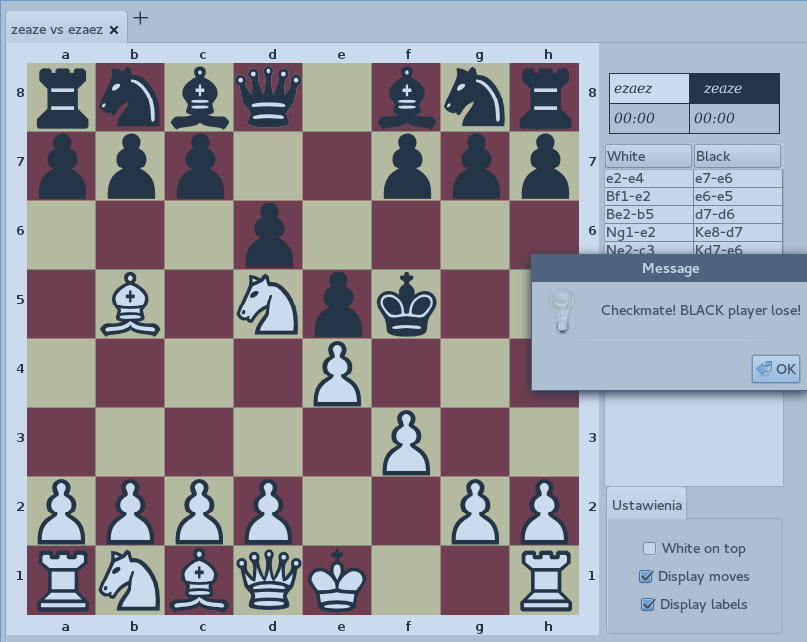
\includegraphics[scale=0.5]{img/Badmat}
		\label{Badmat}
	\end{center}
	Des cas de tests ont été ajoutés dans le fichier de test.

	\section{Monteur pour la visibilité}
	\label{sec:Monteur pour la visibilite}
	Dans le package \emph{jchess.core.Moves}, j'ai décidé de mettre en place un pattern design \emph{Builder} couplé avec un design pattern \emph{Strategy}. Le premier me permet de construire un objet par chaînage. Ainsi les méthodes from/to retournent une instance de ce même objet, comme par exemple~:
	\begin{minted}{java}
		public AlgebricChainMove from(String value)
	\end{minted}
	Ce qui donne en exemple concret~:
	\begin{minted}{java}
		new AlgebricChainMove(board).from("d2").to("d4").move();
	\end{minted}
	De plus, le second pattern permet de choisir la solution d'écriture de mouvement que l'on souhaite. On a le choix entre 2 méthodes. \emph{AlgebricChainMove} et \emph{NumericChainMove}. Les 2 solutions utilisent la méthode move définie dans la classe abstraite. \emph{MoveBuilder}.

	\section{Variantes}
	\label{sec:Variantes}

	Pour la variante des tailles, il a falu reprendre la gestion de la taille de l'échequier un peu partout dans le code en modifiants les tailles hardcodées en \emph{chessboard.getSize()}.\\
	La nouvelle pièce (Arrow) créée a été définie sur le même modèle que toutes les autres pièces (dans les packages \emph{piece} et \emph{behavior}).\\
	Un pattern \emph{Strategy} a été implémenté pour le choix du mode. 3 modes ont été développés (Mode classique (où il faut une taille de 8), mode aléatoire (n'importe quelle taille) et mode pions (n'importe quelle taille)). Chaque mode hérite d'une classe abstraite \emph{jchess.core.setpieces.SetPieces} et implémente la méthode~:
	\begin{minted}{java}
		public abstract void setPieces4NewGame(Player plWhite, Player plBlack);
	\end{minted}
	\begin{center}
		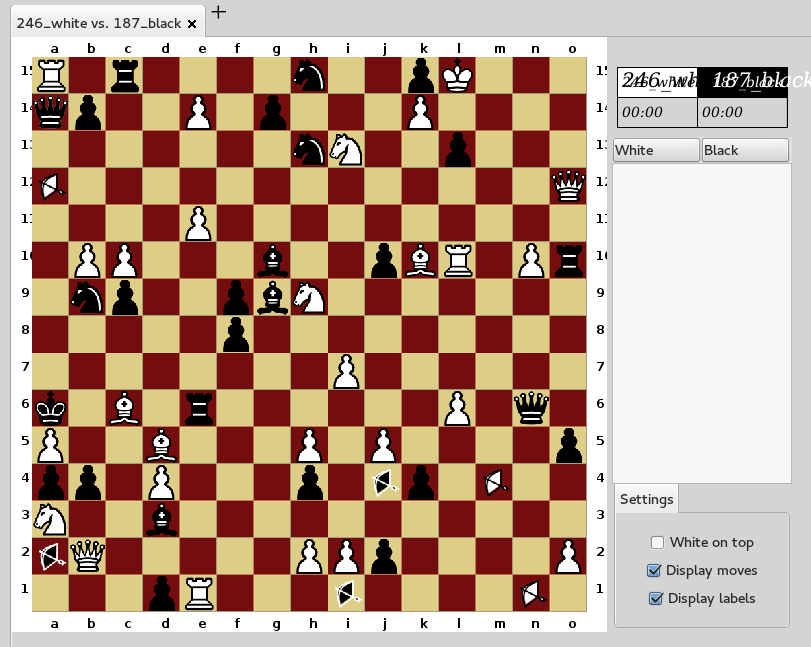
\includegraphics[scale=0.5]{img/Variantes}
		\label{Variantes}
	\end{center}

	\section{En visite}
	\label{sec:En visite}
	Dans le package \emph{jchess.core.visitor}, on peut voir l'implémentation d'un design pattern \emph{Visitor} là-aussi couplé avec un design pattern \emph{Strategy} pour le choix du type de Visiteur. Ainsi chaque visiteur (ici \emph{ScoringVisitor} et \emph{TypeVisitor}) doit implémenter les méthodes~:
	\begin{minted}{java}
		void visit(Chessboard chessboard);
		void visit(Square square);
	\end{minted}
	qui seront ordonnées par les méthooes accept~:
	\begin{minted}{java}
		//Dans Chessboard.java
		public void accept(ChessboardVisitor visitor) {
			for (int i = 0; i < settings.getSize(); i++) // create object for each
			// square
			{
				for (int y = 0; y < settings.getSize(); y++) {
					squares[i][y].accept(visitor);
				}
			}
			visitor.visit(this);
		}
		//Dans Square.java
		public void accept(ChessboardVisitor visitor) {
			visitor.visit(this);
		}
	\end{minted}

	\section{Décoration}
	\label{sec:Decoration}
	Ici la classe Move a vu 2 nouveaux attributs, via le design pattern Decorator~:
	\begin{minted}{java}
		private String duration = null;
		private String comment = null;
	\end{minted}
	Qu'on passe en paramètre via la méthode addMove~:
	\begin{minted}{java}
		public void addMove(Square begin, Square end, boolean registerInHistory,
		Castling castlingMove, boolean wasEnPassant, Piece promotedPiece,
		String duration, String comment);
	\end{minted}

	\section{AI}
	\label{sec:AI}
	Ici encore, un design apttern de type \emph{Strategy} a été mis en place pour implémenter les différentes intelligences. Ces classes sont visibles dans le package \emph{jchess.core.computerai}. Ici chaque classe héritant doit implémenter la méthode~:
	\begin{minted}{java}
		public abstract void move(Chessboard board);
	\end{minted}
	De plus, les tests \emph{testGlouton()} et \emph{testAI()} on été implémenté pour cette partie.
	\begin{center}
		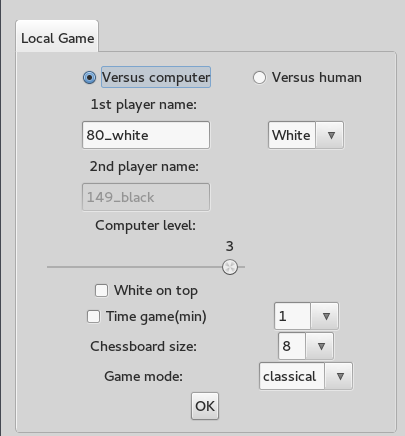
\includegraphics[scale=0.5]{img/AI}
		\label{AI}
	\end{center}

	\section{Bilan}
	\label{sec:Bilan}
	Le diagramme UML du projet étant plutôt massif, il ne sera pas inclu directement dans ce rapport. Vous pouvez le trouver à l'url suivante~: \url{https://github.com/AmarOk1412/ChessMDI/blob/master/uml/final.png?raw=true}.\\
	Dans ce projet, j'ai mis en place quelques design pattern comme \emph{Singleton} (Section \ref{sec:Au commencement}), \emph{Strategy} (Section \ref{sec:AI}), \emph{Builder} (Section \ref{sec:Monteur pour la visibilite}), \emph{Visitor} (Section \ref{sec:En visite}) et \emph{Decorator} (Section \ref{sec:Decoration}).\\
	Au final, beaucoup de choses n'étaient pas bien implémenté au début et des fonctionnalités plantaient (bug de déplacement, de promotion, de mise en échec, de logging, des tests manquants, etc). La partie la moins compréhensible était le lancement de l'application où on ne voyait pas comment il lançait l'application.

\end{document}
